\documentclass{beamer}
\usepackage[utf8]{inputenc}
\usepackage[T1]{fontenc}

\usetheme{Cuerna}
\usecolortheme{default}

% slide (frames) numbering
\addtobeamertemplate{navigation symbols}{}{
    \usebeamerfont{footline}%
    \usebeamercolor[fg]{footline}%
    \hspace{1em}%
    \insertframenumber
}

\title{Adversarial Attacks on Neural Network Policies}
\author{Shayan Amani\\}

\date{spring 2019}
\institute{RLRL Weekly Group Meeting}

\begin{document}

  \begin{frame}
    \titlepage
  \end{frame}
  
\begin{frame}{In This Paper}

Tampering input of the mentioned models with barely perceptible piece of information could lead to fooling the agent to take actions which amount to reduced final return (reward).

\begin{itemize}
    \item 3 type of attacks
    \item 3 methods
    \item 3 constraints
    \item 4 benchmark games
\end{itemize}
    
\end{frame}
 
\begin{frame}{Adversarial Attacks}
Adversarial attacks fall in either one of the following categories based upon the stage which in the adversary perturbs the model:
\begin{itemize}
    \item Train time: Data poisoning.
    \item Evaluation time: Adversarial examples.
    \item Deploy time: Black-box attacks.
\end{itemize}
    
\end{frame}

\begin{frame}{Contributions}
Contribution of this paper can be framed into two form of attacks to state-of-the-art methods, A3C, TRPO, and DQN. Inspired by cryptography and cyber attacks, they are named as follows:
\begin{itemize}
    \item \textbf{White-box attacks}: adversary has access to the model under-the-hood.
    \item \textbf{Black-box attacks}: adversary has no knowledge about the model.
\end{itemize}

\end{frame}

\begin{frame}
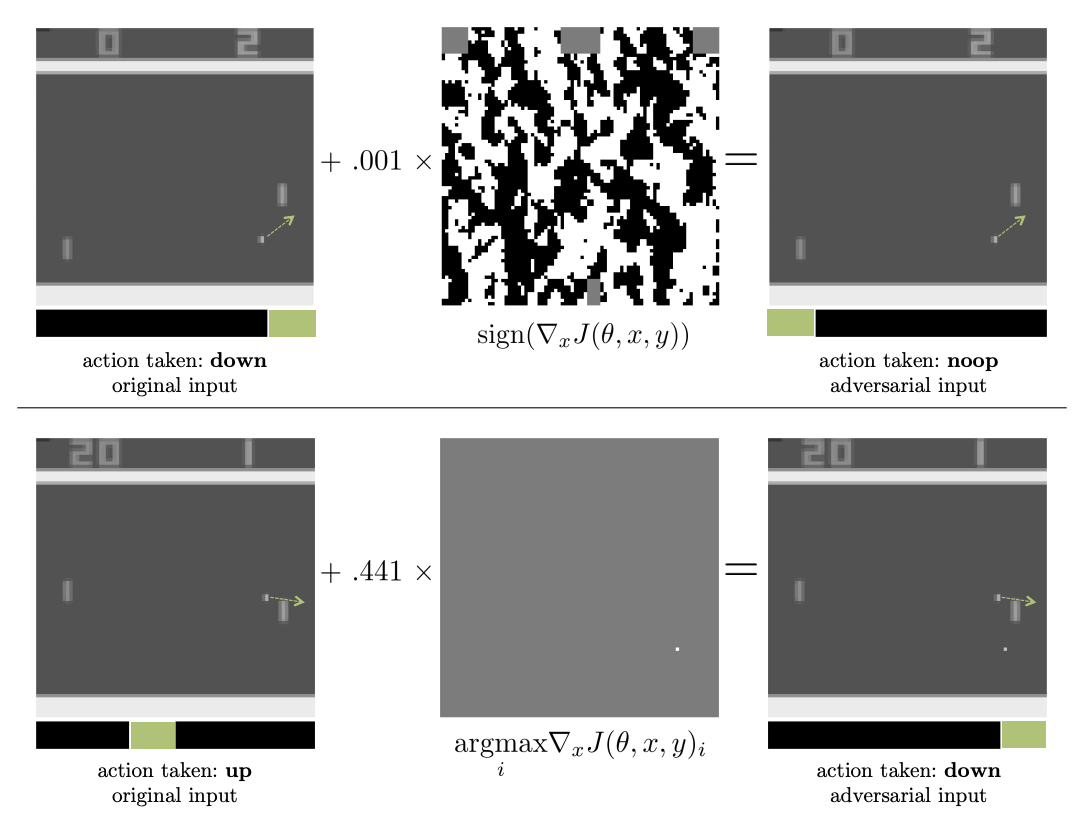
\includegraphics[width= 1\columnwidth]{fig1-l-inf-vs-l-1.png}
\end{frame}


\begin{frame}{Effect of Norm}
The paper has also reviewed effect of constraining three mentioned methods with $\ell_\infty$, $\ell_2$, and $\ell_1$ -norms.

\end{frame}

\begin{frame}
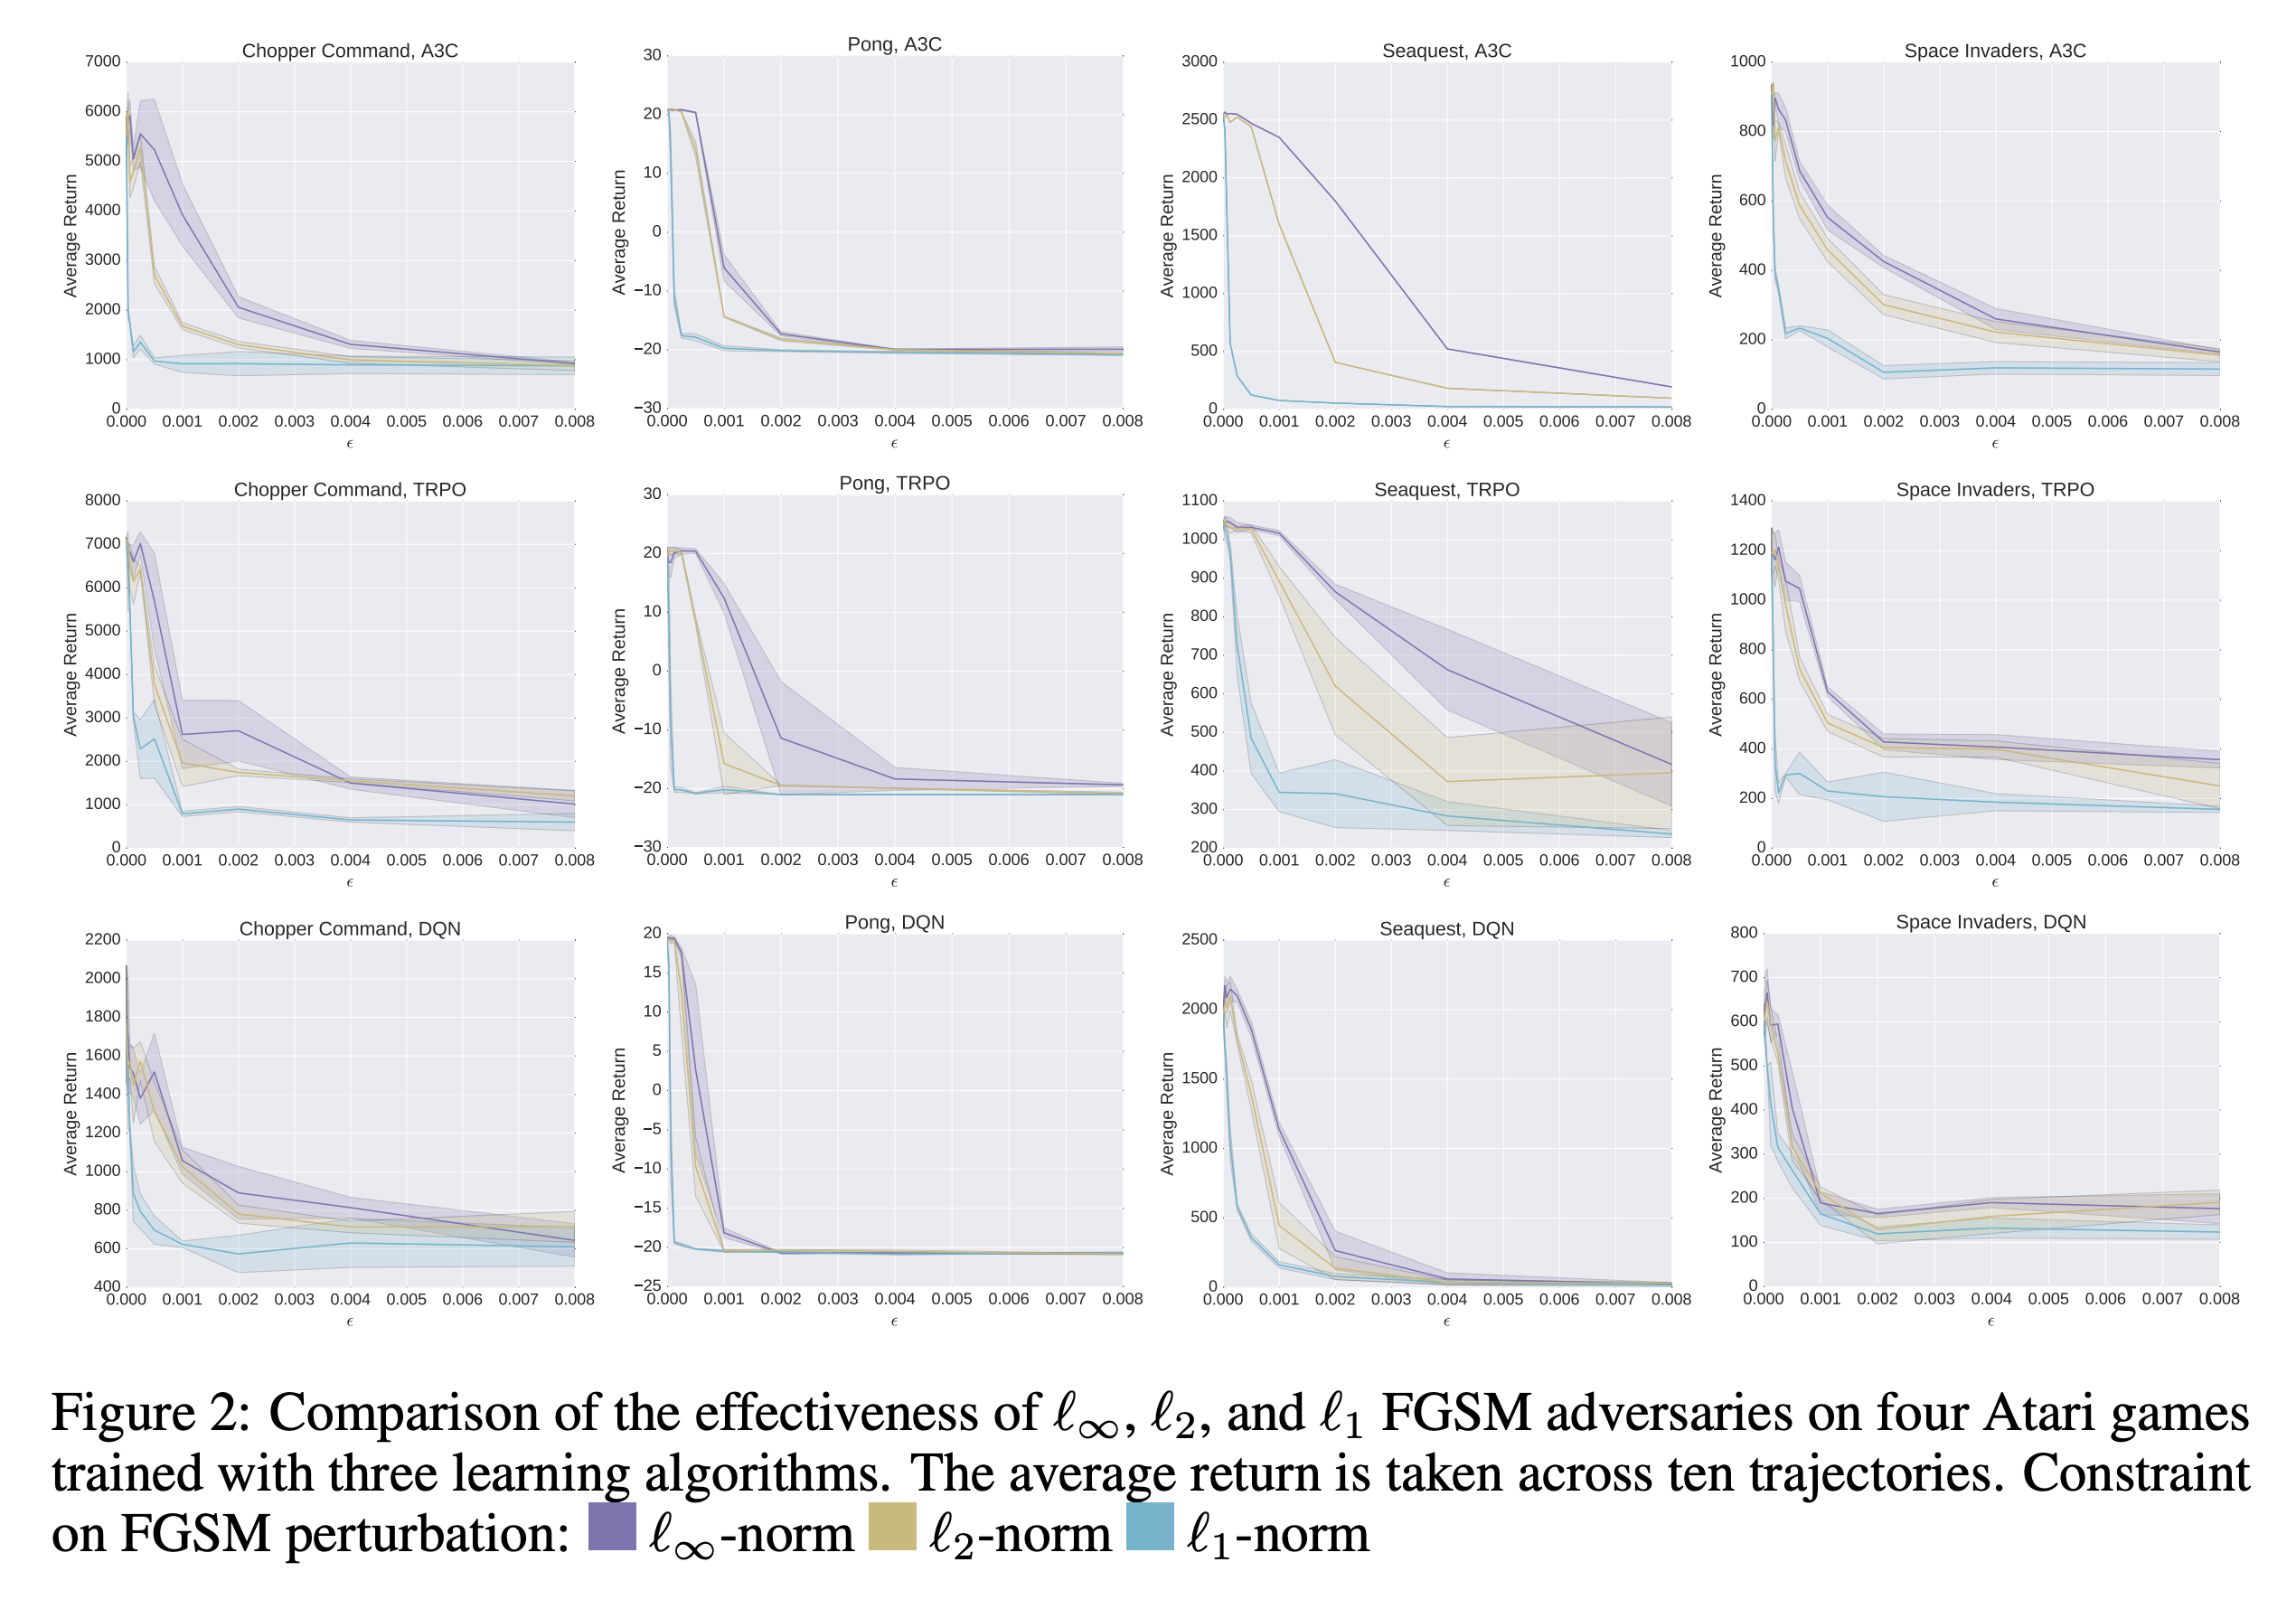
\includegraphics[width =1\columnwidth]{fig2-diff-norms.png}
\end{frame}

\begin{frame}
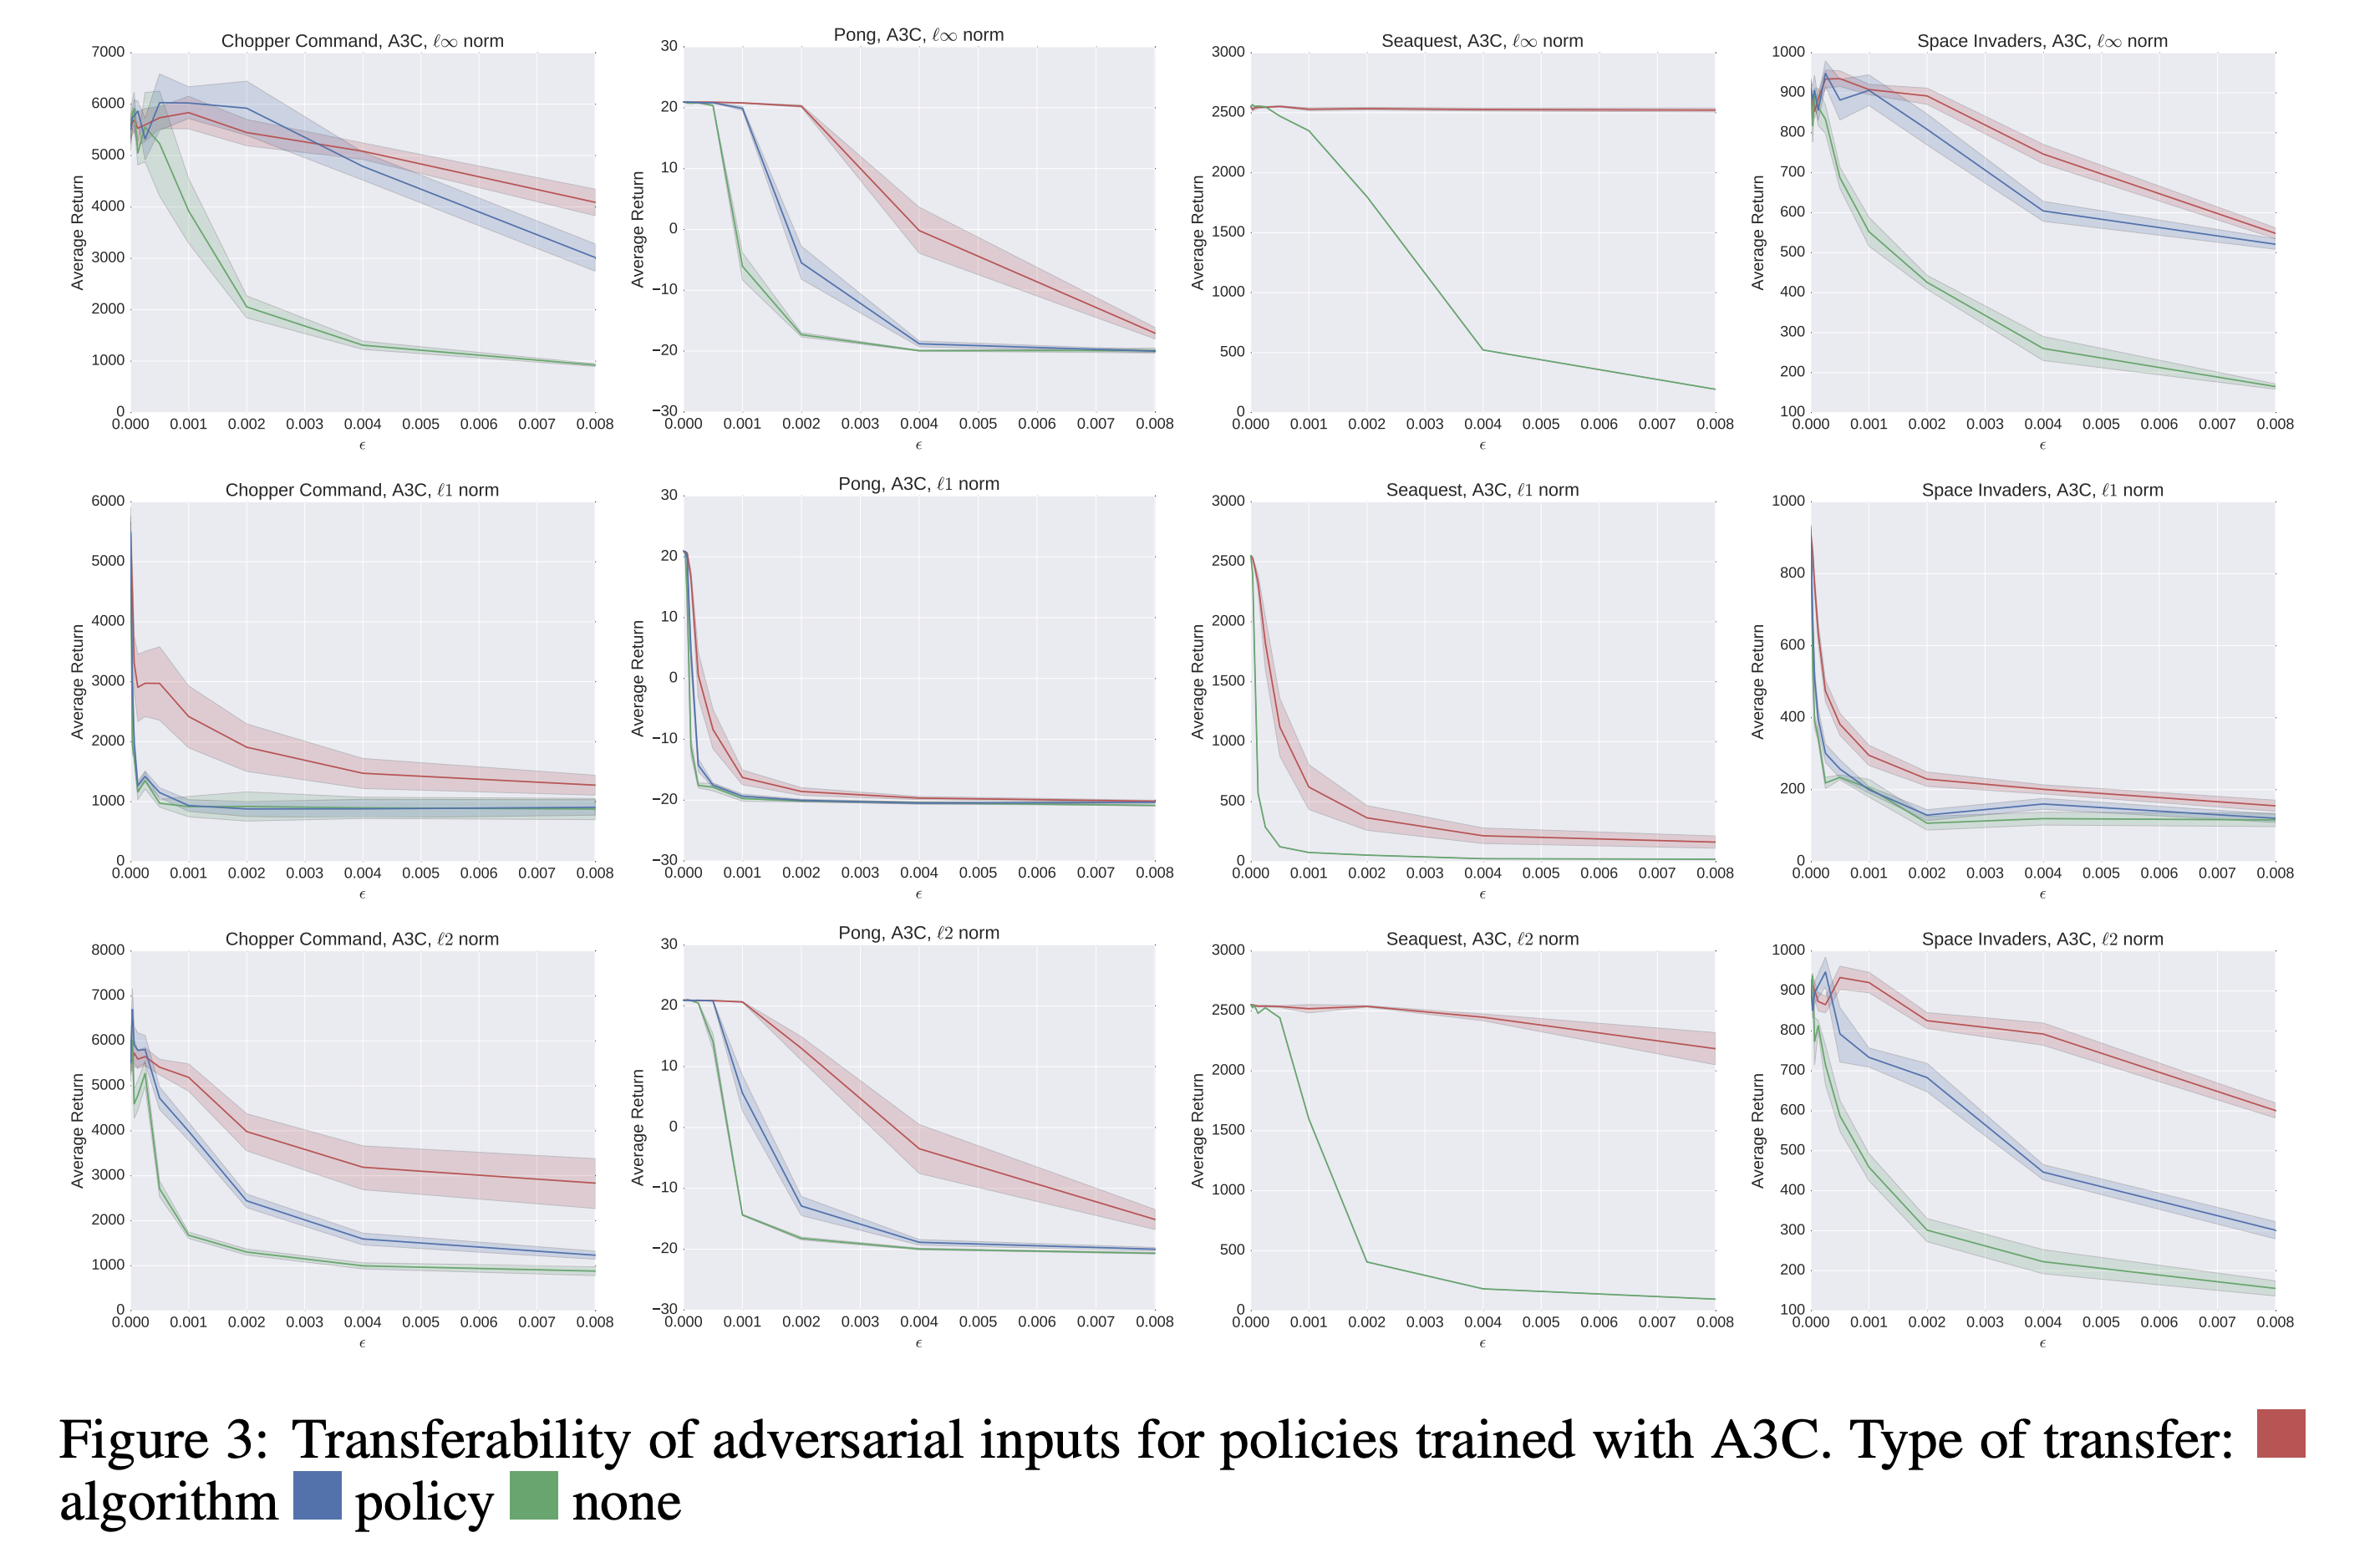
\includegraphics[width =1\columnwidth]{fig3-trans-A3C.png}
\end{frame}

\begin{frame}
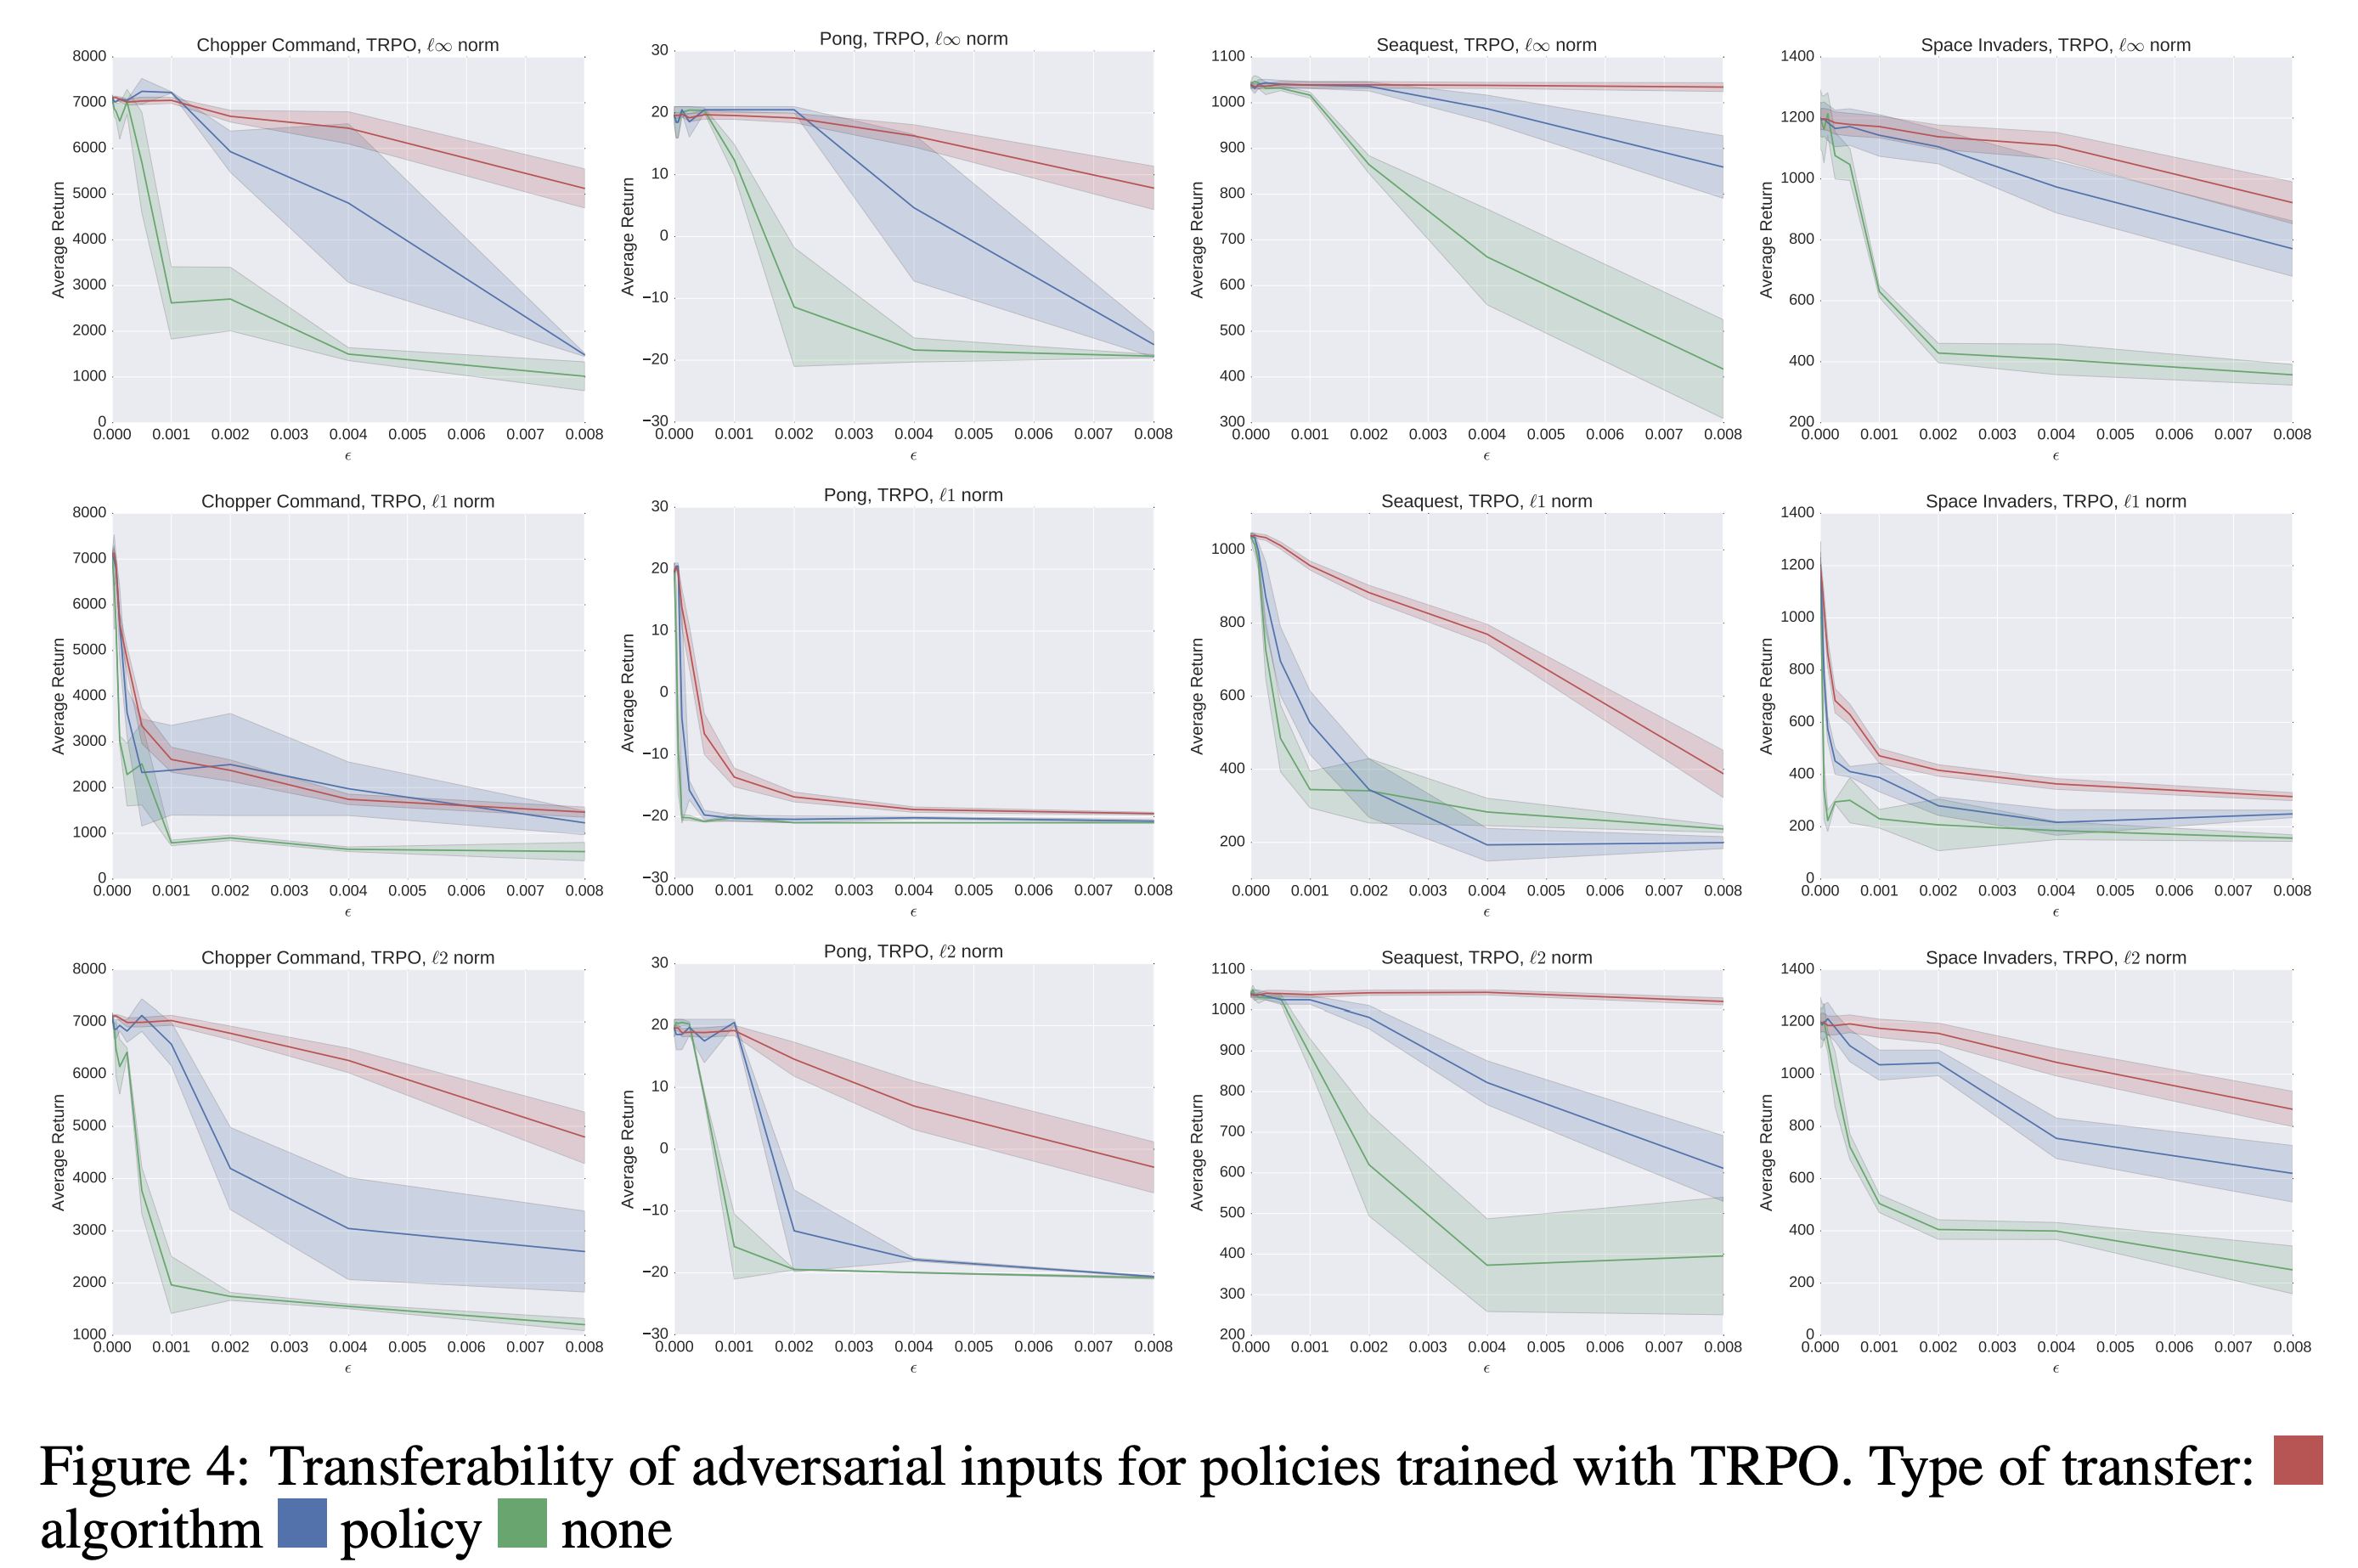
\includegraphics[width =1\columnwidth]{fig4-trans-TRPO.png}
\end{frame}

\begin{frame}
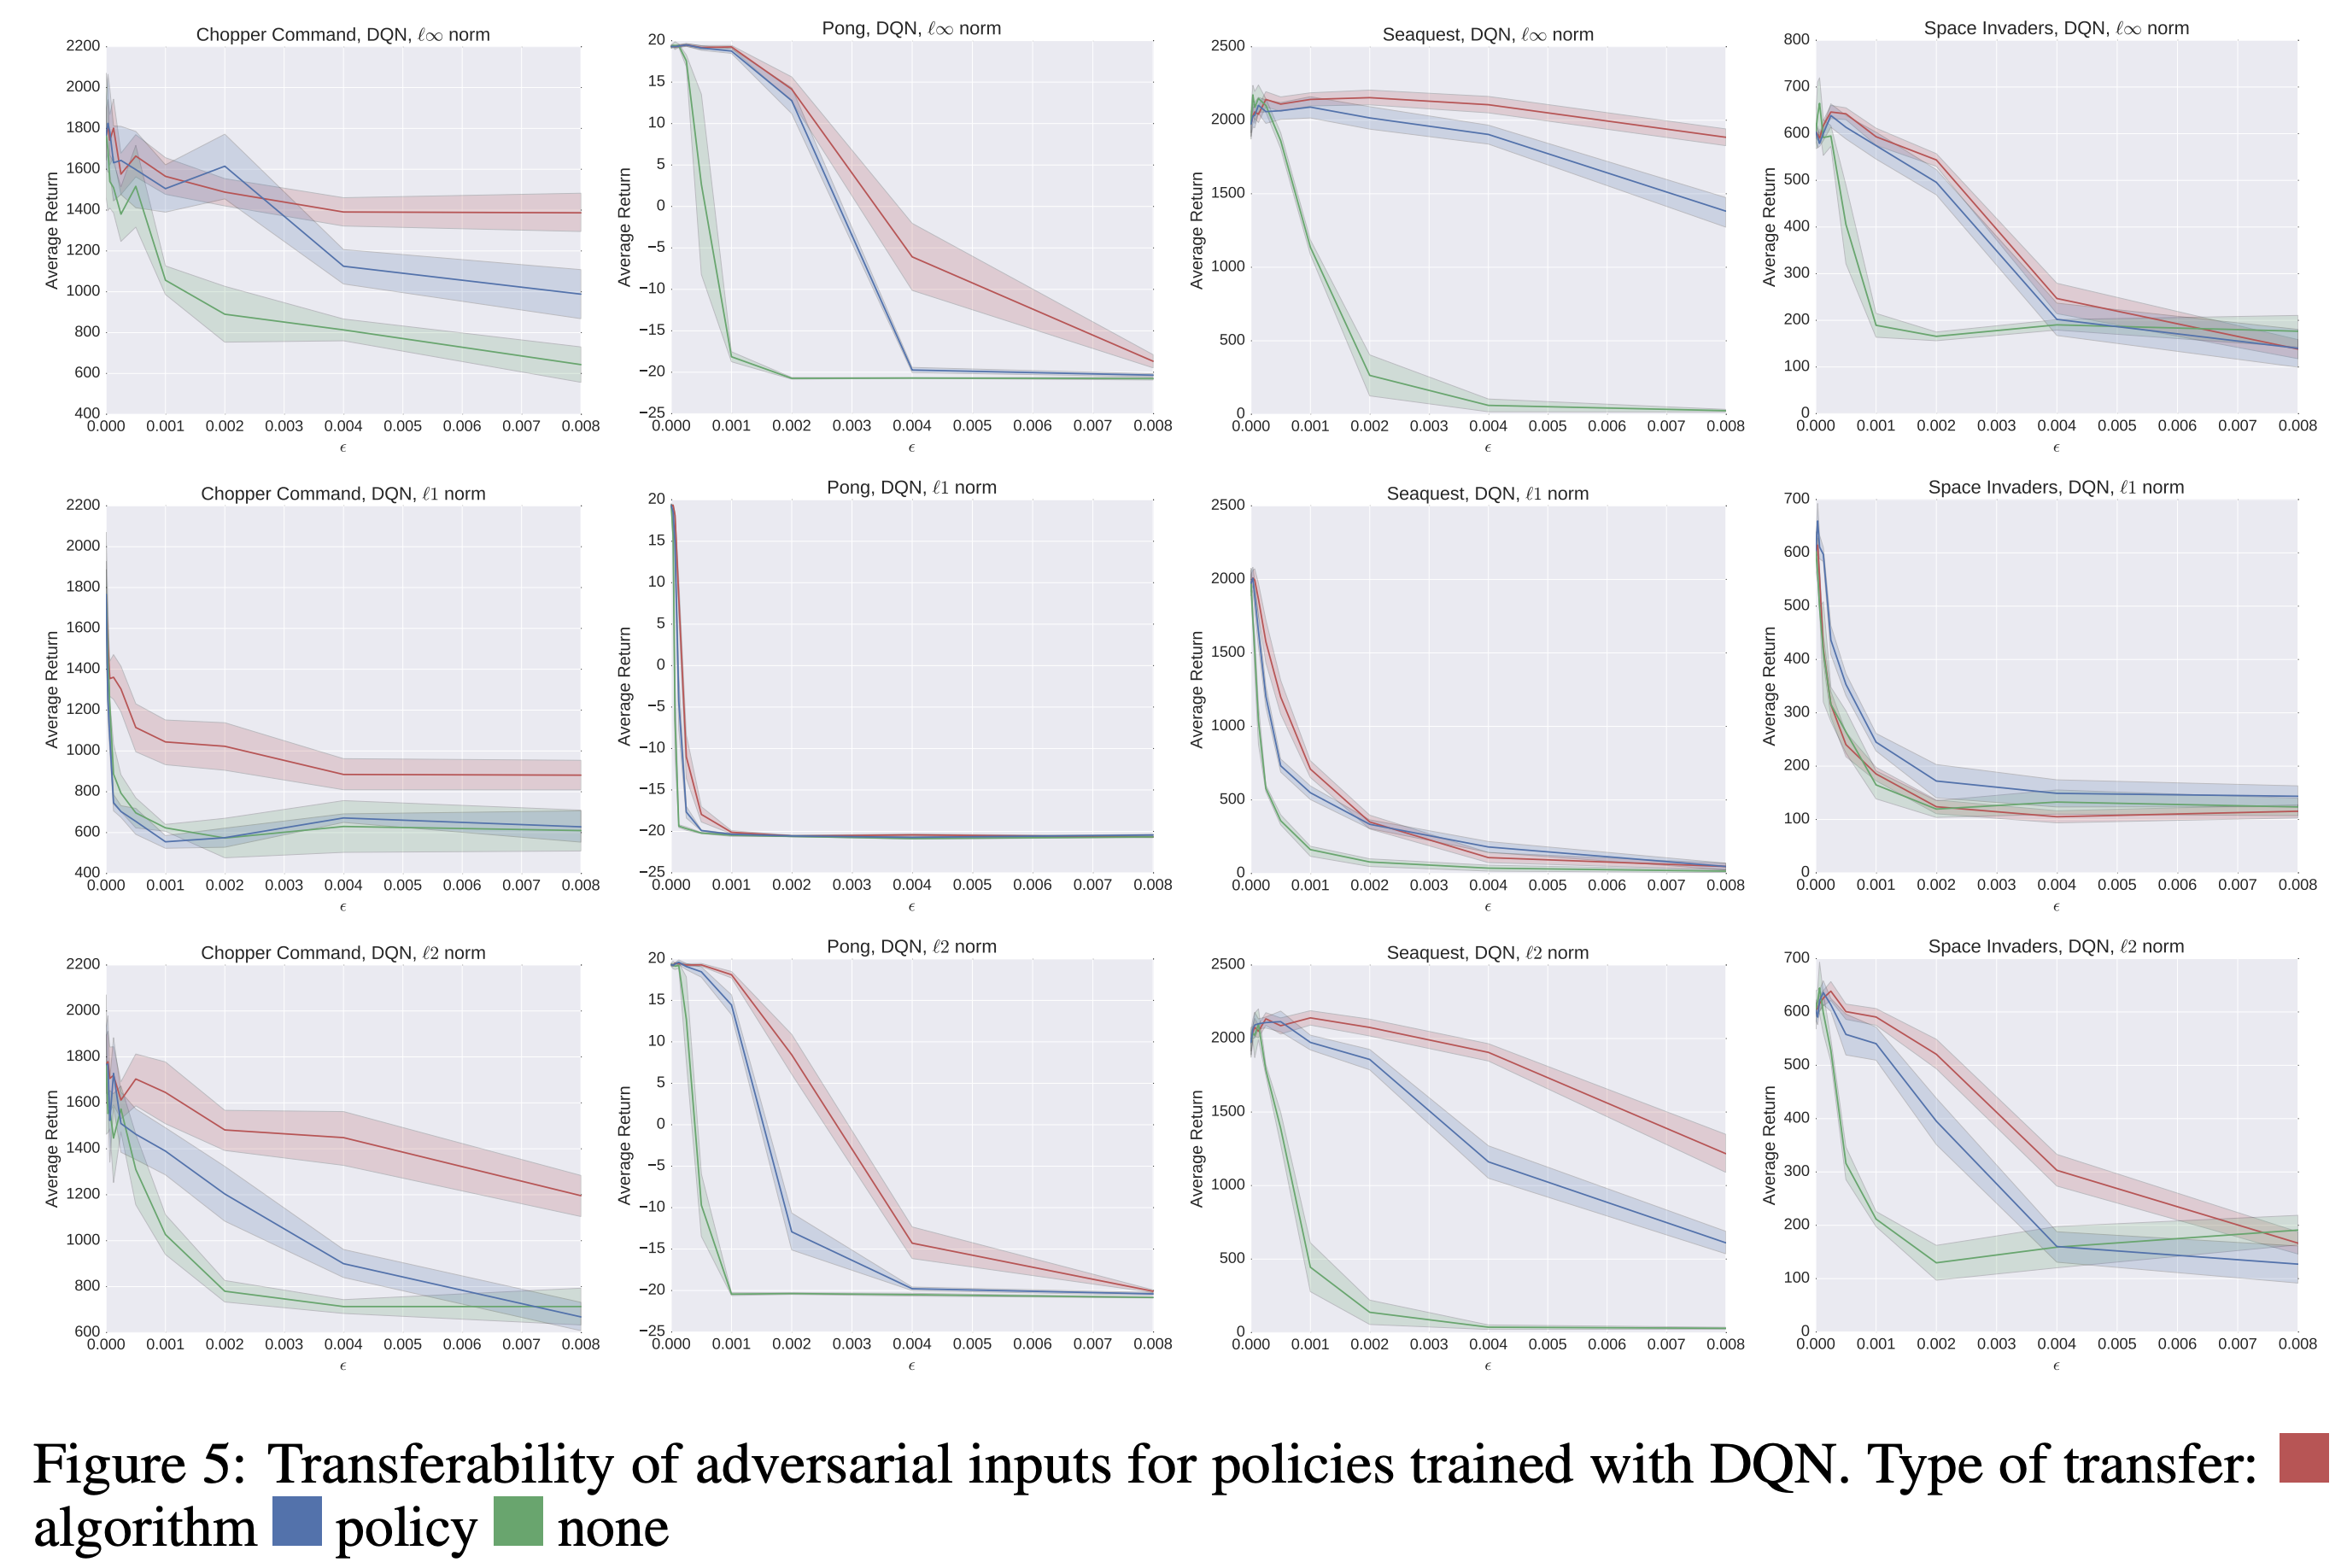
\includegraphics[width =1\columnwidth]{fig5-trans-DQN.png}
\end{frame}

\end{document}